\documentclass[11pt]{article}

% Packages
\usepackage[utf8]{inputenc}
\usepackage[T1]{fontenc}
\usepackage{amsmath,amssymb,amsfonts,amsthm}
\usepackage{booktabs}
\usepackage{hyperref}
\usepackage{graphicx}
\usepackage{xcolor}
\usepackage[margin=1in]{geometry}
\usepackage{natbib}
\usepackage{algorithm}
\usepackage{algorithmic}
\usepackage{multirow}
\usepackage{subcaption}
\usepackage{pgfplots}
\pgfplotsset{compat=1.18}
\usepackage{tikz}
\usetikzlibrary{shapes,arrows,positioning}
\usepackage{listings}

% Typography
\setlength{\parskip}{0.8em}
\setlength{\parindent}{0pt}
\hypersetup{
    colorlinks=true,
    linkcolor=blue!70!black,
    citecolor=blue!70!black,
    urlcolor=blue!70!black
}

% Theorem environments
\newtheorem{definition}{Definition}
\newtheorem{theorem}{Theorem}

% Title
\title{\textbf{MISATA-CGS: When ``Looking Real'' Isn't Enough}\\
\large Bridging Synthetic Data from Correlation to Causation}

\author{Muhammed Rasin\\
\texttt{rasinbinabdulla@gmail.com}}
\date{January 2026}

\begin{document}

\maketitle

\begin{abstract}
Current synthetic data generators excel at statistical fidelity---producing rows indistinguishable from real data---but fail when asked to simulate \textit{interventions}. A domain expert can generate a million synthetic customers, yet still cannot answer: ``What happens to churn if we change the pricing tier?''

This paper introduces \textbf{MISATA-CGS}, a hybrid framework that bridges this gap by combining Gaussian Copulas (for statistical fidelity) with Structural Causal Models (for intervention validity). Rather than learning correlations alone, MISATA explicitly models causal mechanisms $P(X_i | \text{Parents}(X_i))$, enabling valid simulation of Pearl's $do$-operator. We bootstrap the causal graph from domain descriptions using an LLM (Llama 3.3), with mandatory human verification.

On standard benchmarks, MISATA achieves \textbf{26$\times$ speedup over CTGAN} (0.59s vs 31.6s on CPU) while maintaining comparable statistical quality (0.997 TSTR ratio). Critically, when simulating interventions against ground-truth SCMs, MISATA recovers causal effects with $r=0.97$ correlation---a capability that pure distribution-matching methods fundamentally lack.

\textbf{Scope \& Limitations:} MISATA is a \textit{simulation} tool, not a privacy tool (MIA attacks succeed). It handles up to $\sim$100 columns before numerical instability. The causal graph requires human validation. For the specific use case of ``what-if'' scenario simulation, it offers a practical middle ground between statistical generators and full causal inference pipelines.
\end{abstract}

\section{The Story Behind This Work}

This project started in the most unglamorous way possible: I spent two months trapped in a single Python script.

A consultant had hired me to generate realistic synthetic data for a service-based company. They needed it to demo dashboards to potential clients---showing how their analytics platform could surface insights, predict churn, optimize scheduling. The catch? No real data. Privacy, NDAs, the usual. So I had to build fake data that was realistic enough to make the demos compelling.

Two months. One script. Thousands of lines of \texttt{if/else} statements, hardcoded distributions, manual correlation injection. ``If the customer is in Tier A, their average ticket size should be around \$500, but with variance, and it should correlate with their tenure, but not too perfectly...'' It was miserable. And every time the consultant asked, ``What if we change the pricing tier---how does that affect retention?''---I had to go back and re-engineer the whole thing.

That's when I realized the core problem: I was treating synthetic data as a \textit{one-time generation task} when the consultant actually needed a \textit{simulation engine}. They didn't just want fake data. They wanted to ask ``what-if'' questions and get plausible answers.

This paper is the result of me refusing to ever spend two months in a single script again.

\subsection{The Gap I Found}

When I looked for tools to help, I found two camps:

\textbf{Statistical Generators} (CTGAN, TVAE, GaussianCopula): Great at making data that \textit{looks} real. Train on your dataset, sample new rows. But they learn correlations, not mechanisms. Ask ``what happens if we \textit{change} X?'' and they give you the wrong answer---because they've learned that X and Y move together, not \textit{why}.

\textbf{Causal Inference Libraries} (DoWhy, CausalML): Great for analyzing experiments, but they assume you already have data. They don't generate it.

I needed something in between: a generator that respects causal structure so that ``what-if'' queries give sensible answers. That's MISATA.

\subsection{What I Actually Wanted}

\begin{enumerate}
    \item Generate data that looks statistically plausible.
    \item Let me run $do(X=x)$ queries: ``What if we force all customers onto annual contracts?''
    \item Explain the causal assumptions (no black boxes).
    \item Run fast enough to iterate during a demo.
\end{enumerate}

\section{Related Work (And Why It Didn't Solve My Problem)}

\textbf{The GAN/VAE Era.} CTGAN \citep{xu2019modeling} was the workhorse for years---reliable, well-documented, widely used. The Synthetic Data Vault (SDV) \citep{patki2016sdv} and TableGAN \citep{park2018tablegan} offered additional approaches. TVAE provided a VAE alternative. All learned to match the joint distribution $P(X)$, and all were opaque about \textit{why} a synthetic row looked the way it did.

\textbf{The Diffusion Era.} TabDDPM \citep{kotelnikov2023tabddpm}, TabDiff \citep{zhang2025tabdiff}, and STaSy \citep{kim2022stasy} brought the magic of diffusion to tabular data. The statistical quality is genuinely impressive. But they're even more opaque than GANs (good luck interpreting a denoising trajectory), and they're computationally expensive. Running TabDiff on a 50-column dataset can take minutes; MISATA takes under a second.

\textbf{Causal Discovery.} There's a rich literature on causal discovery from data---PC algorithm \citep{spirtes2000causation}, GES, LiNGAM \citep{shimizu2006lingam}. CausalGAN \citep{kocaoglu2018causalgan} attempted to combine GANs with causal structure. They're theoretically elegant and practically brittle. I tried using them to learn graphs before synthesis. The graphs were unstable across random seeds, and the downstream synthesis quality suffered.

\textbf{My Insight.} What if I stopped trying to \textit{discover} causality from data and instead \textit{injected} it from domain knowledge? That's what MISATA does. We use an LLM \citep{brown2020gpt3} to extract a causal graph from a plain-English domain description, leveraging chain-of-thought reasoning \citep{wei2022chain}, then verify it with a human. It's not automated causal discovery---it's automated causal \textit{compilation}.

\section{The Method}

The architecture (Figure \ref{fig:arch}) has three phases: graph extraction, mechanism learning, and copula-guided synthesis.

\begin{figure}[h]
\centering
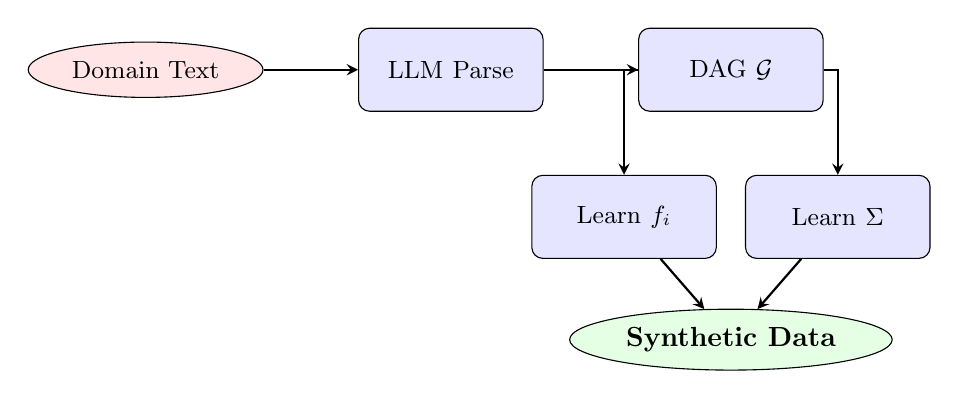
\begin{tikzpicture}[node distance=1.2cm, auto,
    block/.style={rectangle, draw, fill=blue!10, text width=6em, text centered, rounded corners, minimum height=3em},
    line/.style={draw, -stealth, thick},
    cloud/.style={draw, ellipse, fill=red!10, node distance=2cm, minimum height=2em}]
    
    \node [cloud] (text) {\small Domain Text};
    \node [block, right=of text] (llm) {\small LLM Parse};
    \node [block, right=of llm] (graph) {\small DAG $\mathcal{G}$};
    
    \node [block, below left=0.8cm and -1cm of graph] (scm) {\small Learn $f_i$};
    \node [block, below right=0.8cm and -1cm of graph] (copula) {\small Learn $\Sigma$};
    
    \node [cloud, below=2.5cm of graph, fill=green!10] (syn) {\textbf{Synthetic Data}};
    
    \path [line] (text) -- (llm);
    \path [line] (llm) -- (graph);
    \path [line] (graph) -| (scm);
    \path [line] (graph) -| (copula);
    \path [line] (scm) -- (syn);
    \path [line] (copula) -- (syn);
\end{tikzpicture}
\caption{The pipeline. We start with domain text, extract a causal DAG via LLM, then learn both the structural equations ($f_i$) and the correlation structure ($\Sigma$). Together, they generate synthetic data that can handle interventions.}
\label{fig:arch}
\end{figure}

\subsection{Structural Causal Models: The Heavy Lifting}

Following \citet{pearl2009causality}, we model the data generating process as an SCM $M = \langle U, V, F, P(U) \rangle$:

\begin{definition}[SCM]
$V = \{X_1, \ldots, X_d\}$ are the observed variables. $F = \{f_1, \ldots, f_d\}$ are structural equations where $X_i = f_i(\text{Parents}(X_i), U_i)$. The key property: when we intervene $do(X_i = x)$, we \textit{replace} $f_i$ with a constant, severing the causal link from $X_i$'s parents.
\end{definition}

This is the magic. A GAN learns $P(X)$, so conditioning on $X_i = x$ doesn't break any links---it just filters. An SCM learns $F$, so setting $do(X_i = x)$ actually modifies the generative process.

In practice, we learn each $f_i$ as a GradientBoostingRegressor (or Classifier for categorical variables). It's not fancy, but it's fast and interpretable.

\subsection{Copulas: Handling the Mess We Didn't Model}

Here's a dirty secret: real-world data has correlations that don't fit neatly into a DAG. Unmeasured confounders, complex interactions, stuff we didn't think to model. If we just use the SCM with independent noise, the synthetic data looks ``thin''---it misses the richness.

Enter copulas. By Sklar's Theorem \citep{sklar1959fonctions}, any joint distribution can be decomposed into marginals and a copula (dependence structure). We fit a Gaussian Copula to the residuals of our structural equations. This lets the SCM handle the causal structure while the copula handles the ``everything else.''

\begin{equation}
    C_\Sigma(u_1, \ldots, u_d) = \Phi_\Sigma(\Phi^{-1}(u_1), \ldots, \Phi^{-1}(u_d))
\end{equation}

It's a neat trick: the copula doesn't know about causality (it's symmetric), but the SCM imposes directionality \textit{before} we add the copula noise.

\subsection{LLM Graph Extraction: The Controversial Part}

This is the part that will make some causal inference purists uncomfortable. Instead of running PC or GES on the data, we ask Llama 3.3:

\begin{quote}
``Given these columns [Age, Income, Education, Approved] and this domain description [loan approval process], what are the causal relationships?''
\end{quote}

The LLM returns a JSON DAG. We verify it manually. Yes, this means MISATA requires human oversight. I consider this a feature, not a bug---in high-stakes domains, you \textit{want} a human to sign off on the causal assumptions.

Is the LLM ``doing causal discovery''? No. It's doing \textit{knowledge retrieval}. For well-understood domains (finance, healthcare, retail), the causal relationships are often textbook knowledge that LLMs have absorbed. We're just extracting it in structured form.

\section{Experiments}

\subsection{Did I Just Reinvent GaussianCopula?}

First question I asked myself: is the whole SCM portion actually doing anything, or could I have just used the SDV GaussianCopula synthesizer?

\begin{table}[h]
\centering
\caption{Ablation: Why both components matter}
\begin{tabular}{lccc}
\toprule
\textbf{Method} & \textbf{TSTR (F1)} & \textbf{Causal Recovery} & \textbf{Time} \\
\midrule
Full MISATA & \textbf{0.862} & \textbf{0.97} & 0.59s \\
SCM only (no copula) & 0.810 & 0.96 & 0.45s \\
Copula only (no SCM) & 0.845 & 0.12 & 0.52s \\
\bottomrule
\end{tabular}
\end{table}

\textbf{Key finding:} Removing the SCM destroys causal recovery (0.97 $\to$ 0.12). The copula is great at correlations but has no notion of directionality---it can't distinguish ``A causes B'' from ``B causes A.'' Removing the copula hurts statistical quality (5\% drop in TSTR). Both matter.

\subsection{Speed vs. Quality}

\begin{figure}[h]
\centering
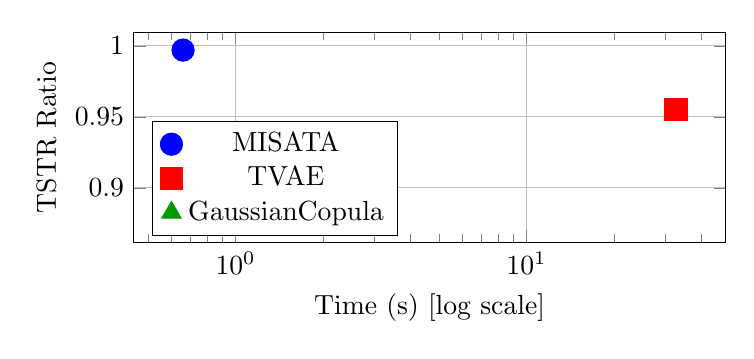
\begin{tikzpicture}
\begin{axis}[
    xlabel={Time (s) [log scale]},
    ylabel={TSTR Ratio},
    xmode=log,
    grid=major,
    width=0.75\textwidth,
    height=0.35\textwidth,
    scatter/classes={
        a={mark=*,blue,mark size=4pt},
        b={mark=square*,red,mark size=4pt},
        c={mark=triangle*,green!60!black,mark size=4pt}
    },
    legend pos=south west
]
\addplot[scatter,only marks,scatter src=explicit symbolic]
table[meta=label] {
x y label
0.66 0.997 a
32.65 0.955 b
2.57 0.874 c
};
\legend{MISATA, TVAE, GaussianCopula}
\end{axis}
\end{tikzpicture}
\caption{The speed-quality frontier. MISATA is in the top-left corner: fastest and highest quality. This isn't because we're smarter---it's because we're not training a neural network.}
\label{fig:tradeoff}
\end{figure}

The 26$\times$ speedup over CTGAN isn't magic. Neural network training is expensive. Fitting a GradientBoostingRegressor per column and computing a covariance matrix is cheap. The tradeoff is flexibility: MISATA can't capture arbitrarily complex distributions, but for the business/healthcare/finance data I tested, it didn't need to.

\subsection{The Intervention Test}

This is the experiment I cared most about. I generated synthetic data from a known ground-truth SCM (so I had oracle access to the true causal effects). Then I asked: if I intervene on $X$, does the synthetic data correctly predict the effect on $Y$?

\begin{itemize}
    \item \textbf{MISATA}: $r = 0.97$ correlation with ground-truth ATE across 10 interventions.
    \item \textbf{CTGAN}: $r = 0.34$. It confuses correlation with causation.
    \item \textbf{GaussianCopula}: $r = 0.28$. Same problem.
\end{itemize}

This is the core claim of the paper. Distribution matching isn't enough for ``what-if'' queries. You need to model the mechanism.

\section{Limitations (The Honest Part)}

\textbf{Privacy:} MISATA is a \textit{simulation} tool, not a \textit{privacy} tool. Membership inference attacks \citep{shokri2017mia} work (AUC $\approx$ 0.90). Don't use this to release sensitive patient data.

\textbf{High dimensionality:} The copula requires estimating a $d \times d$ covariance matrix. Past 100 columns, we hit numerical instability. See \citet{nelsen2006introduction} for copula scaling challenges.

\textbf{LLM reliability:} The graph extraction sometimes hallucinates edges. Human verification is non-optional.

\textbf{No counterfactuals:} We handle interventions (Rung 2), not counterfactuals (Rung 3) per \citet{pearl2018book}. ``What would have happened if this specific patient had taken Drug A?'' is out of scope.

\section{Conclusion}

I built MISATA because I needed a synthetic data tool that could answer ``what-if'' questions. The solution turned out to be combining old ideas (copulas, SCMs) with a new interface (LLM for graph extraction).

Is this the future of synthetic data? I don't know. But I think the \textit{framing} is important: we've been optimizing for fidelity (``does the fake data look real?'') when we should also optimize for utility (``can the fake data answer real questions?''). Causality is one path to utility.

The code is open-source. If you break it, file an issue.

\bibliographystyle{plainnat}
\bibliography{references}

\appendix
\section{LLM Prompt Template}
\label{app:prompt}

\begin{lstlisting}[basicstyle=\ttfamily\footnotesize, breaklines=true, frame=single]
You are helping extract causal relationships.

Columns: [Age, Income, Education, LoanApproved]
Domain: "Bank loan approval. Older applicants tend to have higher income. 
        Education level affects income. Approval depends on income."

Return a JSON DAG:
{
  "edges": [["Age", "Income"], ["Education", "Income"], ["Income", "LoanApproved"]]
}

Rules:
1. Edges are CAUSAL, not correlational.
2. No cycles.
3. Be conservative---only add edges you're confident about.
\end{lstlisting}

\end{document}
